\documentclass{beamer}

\definecolor{myColor1}{rgb}{.97,.91,.81}

\usetheme[progressbar=frametitle]{metropolis}
\useoutertheme{metropolis}
\useinnertheme{metropolis}
\usefonttheme{metropolis}
\usecolortheme{crane}
\setbeamercolor{background canvas}{bg=myColor1}

\title[Algoritmos Computacionales]{Algoritmos Computacionales}
\subtitle{Introducción a la computación}
\author{Víctor de Jesús Medrano Zarazúa \\
	\textit{v.de.jesus@hotmail.com}\\
	\textit{mixlaab.github.io}\\}
\institute{Centro de Educación y Formación Académica}
\date{22 de enero de 2018}

\usepackage[spanish]{babel}
\usepackage[T1]{fontenc}
\usepackage{multicol}
\usepackage{animate}

\begin{document}
	
\begin{frame}
\titlepage
\end{frame}

\begin{frame}[t]{Contenido}\vspace{4pt}
%\begin{multicols}{2}
\tableofcontents
%\end{multicols}
\end{frame}

\section{Definiciones}
\begin{frame}[t]{Definiciones}\vspace{4pt}
\begin{block}{Computadora}
Dispositivo utilizado para procesar información y obtener resulta-
dos.
\end{block}
\begin{multicols}{3}
\begin{figure}
	\centering
	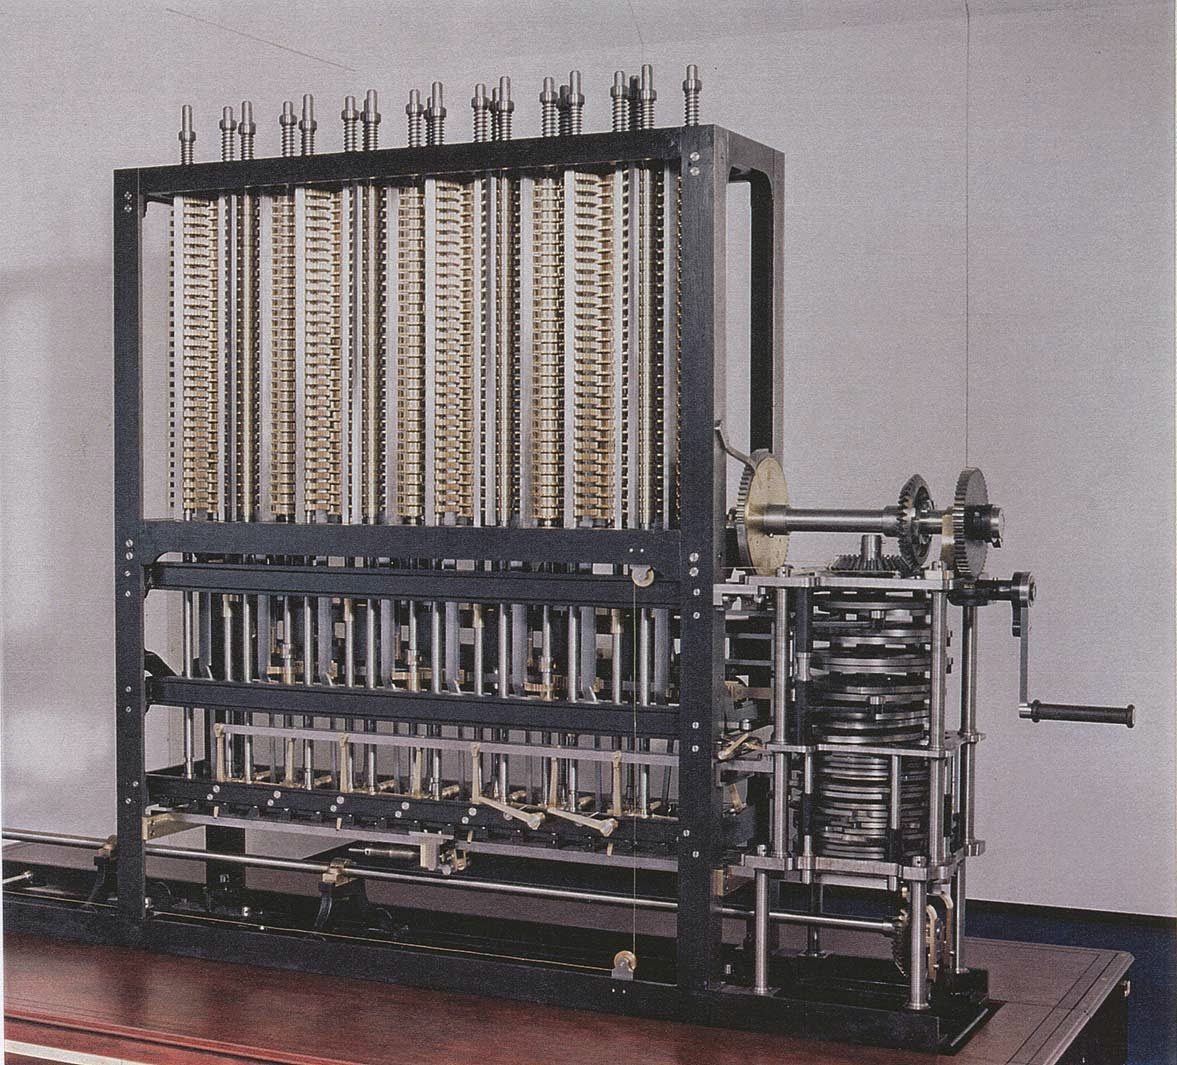
\includegraphics[scale=0.08]{analytical}
	\caption{Máquina analítica}
\end{figure}
\begin{figure}
	\centering
	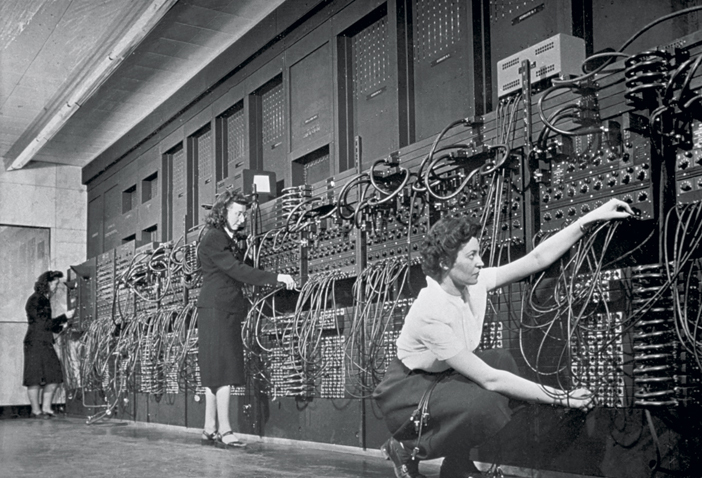
\includegraphics[scale=0.15]{eniac}
	\caption{ENIAC}
\end{figure}
\begin{figure}
	\centering
	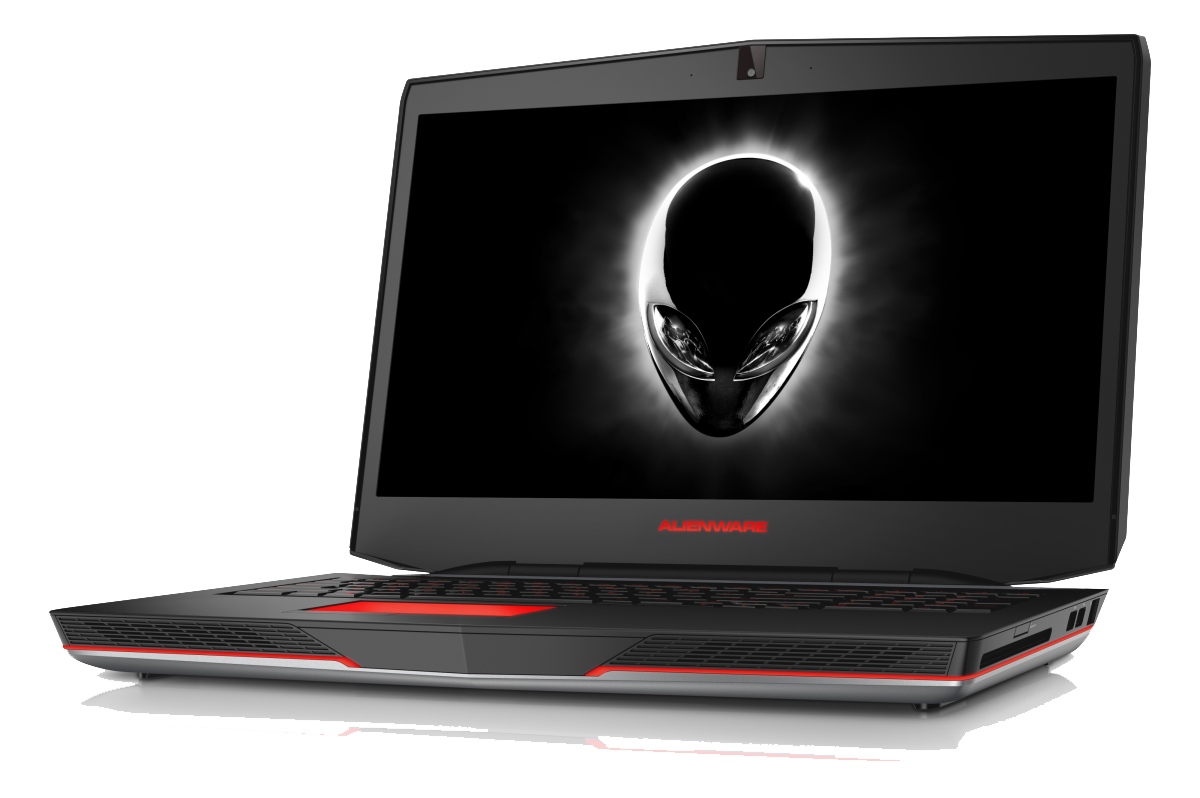
\includegraphics[scale=0.1]{alienware}
	\caption{PC}
\end{figure}
\end{multicols}
\end{frame}

\begin{frame}[t]{Definiciones}\vspace{4pt}
\begin{block}{Hardware}
	Componentes físicos que constituyen la computadora.
\end{block}
\begin{block}{Software}
	Instrucciones con las que se indica a un microprocesador o microcontrolador qué hacer.
\end{block}
\begin{figure}
	\centering
	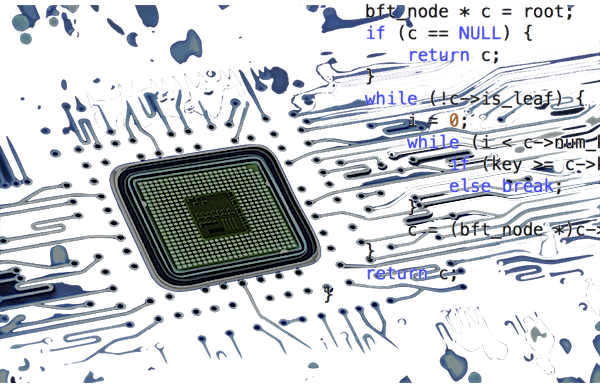
\includegraphics[scale=0.5]{hwsw}
	\caption{Hardware/Software}
\end{figure}
\end{frame}

\begin{frame}[t]{Definiciones}\vspace{4pt}
\begin{block}{Algoritmo}
Secuencia ordenada de instrucciones que conducen a la solución de un problema dado.
\end{block}
\begin{block}{Lenguaje máquina}
Instrucciones escritas en código binario directamente inteligibles por la computadora.
\end{block}
\begin{block}{Lenguaje de alto nivel}
Proporciona un tipo de lenguaje de programación que describe de forma más cercana y más accesible el tipo de operaciones que se requieren.
\end{block}
\end{frame}

\section{Edición y compilación}

\begin{frame}[t]{Edición}\vspace{3pt}
\begin{figure}
	\centering
	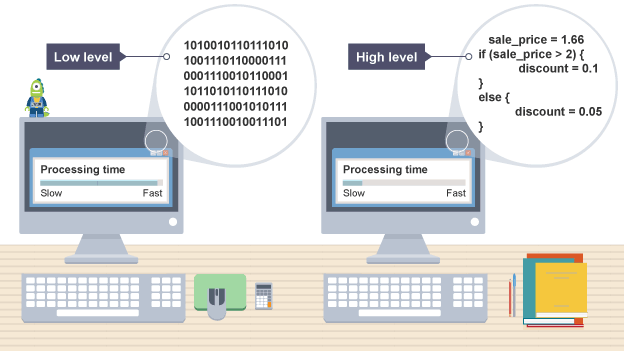
\includegraphics[scale=0.45]{lowhigh}
	\caption{Edición}
\end{figure}
\end{frame}

\begin{frame}[t]{Niveles del lenguaje}\vspace{4pt}
\begin{figure}
	\centering
	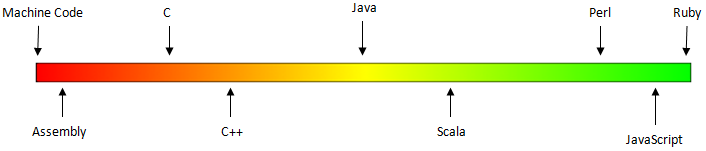
\includegraphics[scale=0.4]{speclang}
	\caption{Lenguajes de programación}
\end{figure}
\begin{multicols}{3}
\begin{figure}
	\centering
	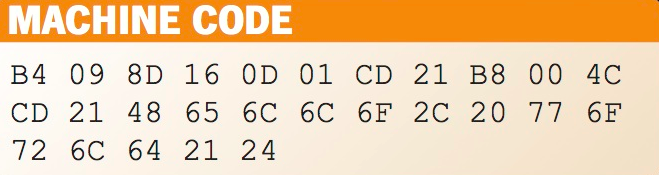
\includegraphics[scale=0.18]{mcode}
	\caption{Lenguaje máquina}
\end{figure}
\begin{figure}
	\centering
	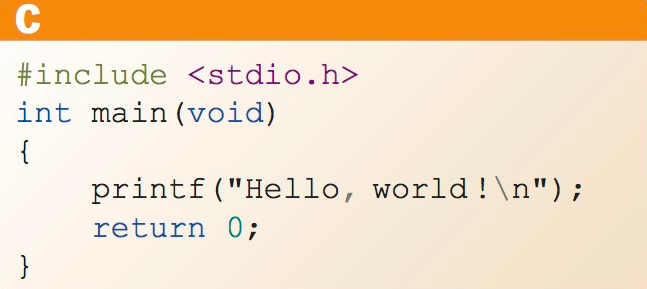
\includegraphics[scale=0.18]{clang}
	\caption{Lenguaje C}
\end{figure}
\begin{figure}
	\centering
	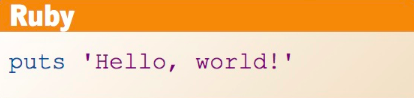
\includegraphics[scale=0.26]{rubylang}
	\caption{Lenguaje Ruby}
\end{figure}
\end{multicols}
\end{frame}

\begin{frame}[t]{Compilación}\vspace{4pt}
\begin{figure}
	\centering
	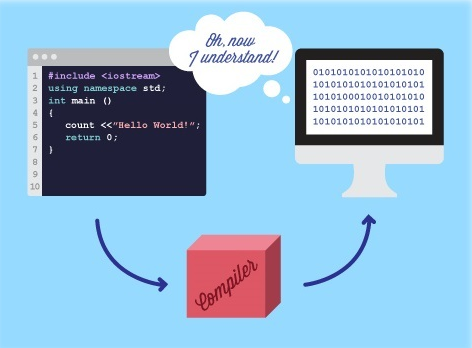
\includegraphics[scale=0.45]{compiler}
	\caption{Compilación}
\end{figure}
\end{frame}

\section{Aplicaciones}

\begin{frame}[t]{Aplicaciones}\vspace{24pt}
\begin{multicols}{3}
\begin{figure}
	\centering
	
\includegraphics[scale=0.2]{softdev}
	\caption{Desarrollo de software}
\end{figure}
\begin{figure}
	\centering
	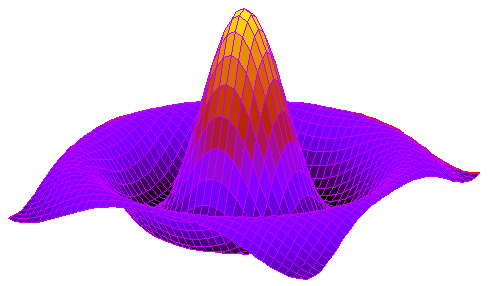
\includegraphics[scale=0.23]{math}
	\caption{Análisis numérico}	
\end{figure}
\begin{figure}
	\centering
	
\includegraphics[scale=0.07]{multimedia}
	\caption{Multimedia}
\end{figure}
\end{multicols}
\end{frame}

\begin{frame}[t]{Aplicaciones}\vspace{24pt}
	\begin{multicols}{3}
		\begin{figure}
			\centering
			
\includegraphics[scale=0.07]{webdesign}
			\caption{Diseño web}
		\end{figure}
		\begin{figure}
			\centering
			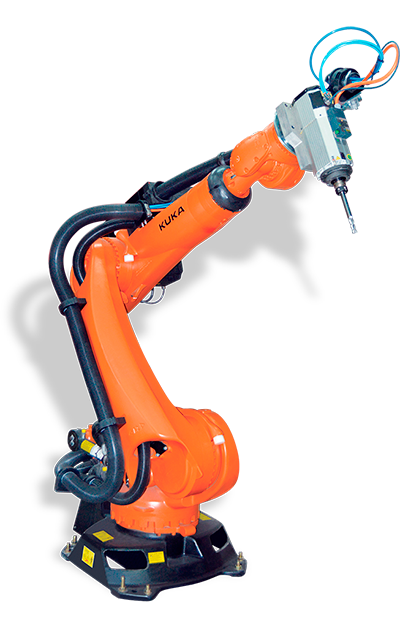
\includegraphics[scale=0.23]{industry}
			\caption{Industria}	
		\end{figure}
		\begin{figure}
			\centering
			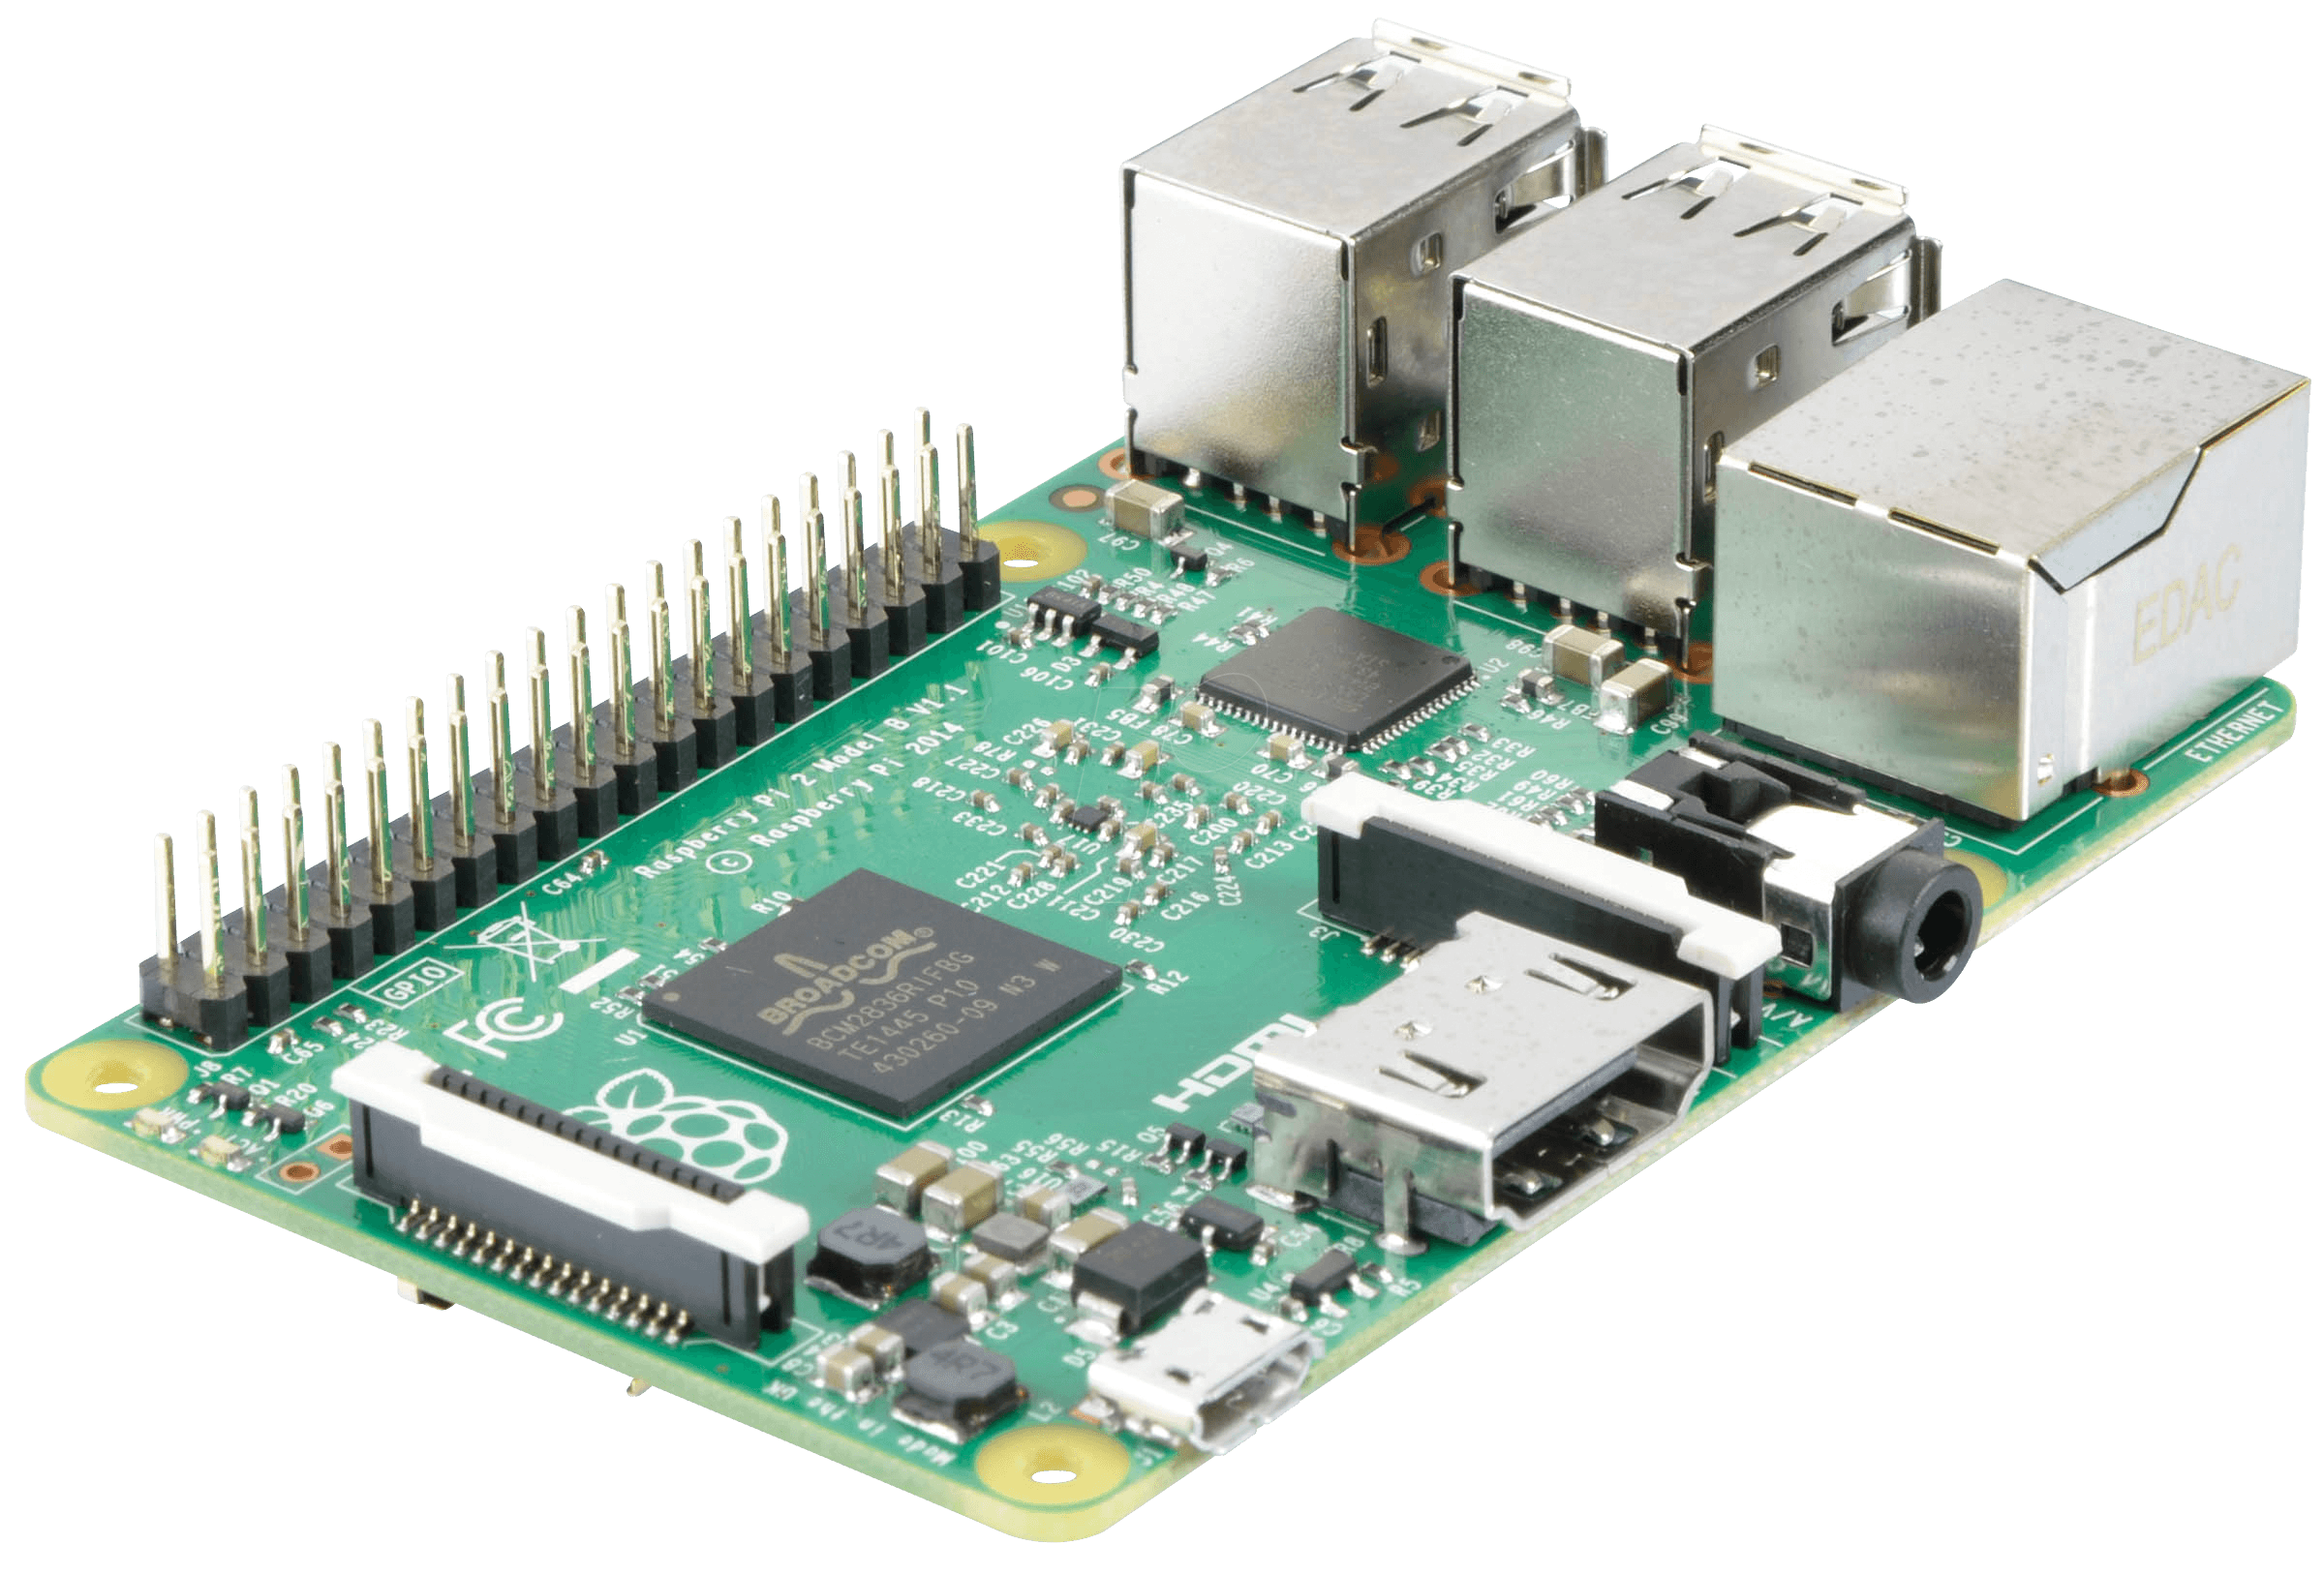
\includegraphics[scale=0.045]{embedded}
			\caption{Sistemas Embebidos}
		\end{figure}
	\end{multicols}
\end{frame}

\section{Historia}
\begin{frame}[t]{Personajes relevantes}\vspace{4pt}
\begin{multicols}{2}
\begin{enumerate}
	\item Ada Lovelace
	\onslide<2->{
	\item Herman Hollerith}
	\onslide<3->{
	\item Alan Turing}
	\onslide<4->{
	\item John von Neumann}
	\onslide<5->{
	\item Dennis Ritchie}
	\onslide<6->{
	\item Bjarne Stroustrup}
	\onslide<7->{
	\item Bill Gates}
	\onslide<8->{
	\item Tim Berners-Lee}
	\onslide<9->{
	\item Linus Torvalds}
	\onslide<10->{
	\item Guido Van Rossum}
\end{enumerate}
\only<1>{
\begin{figure}
	\centering
	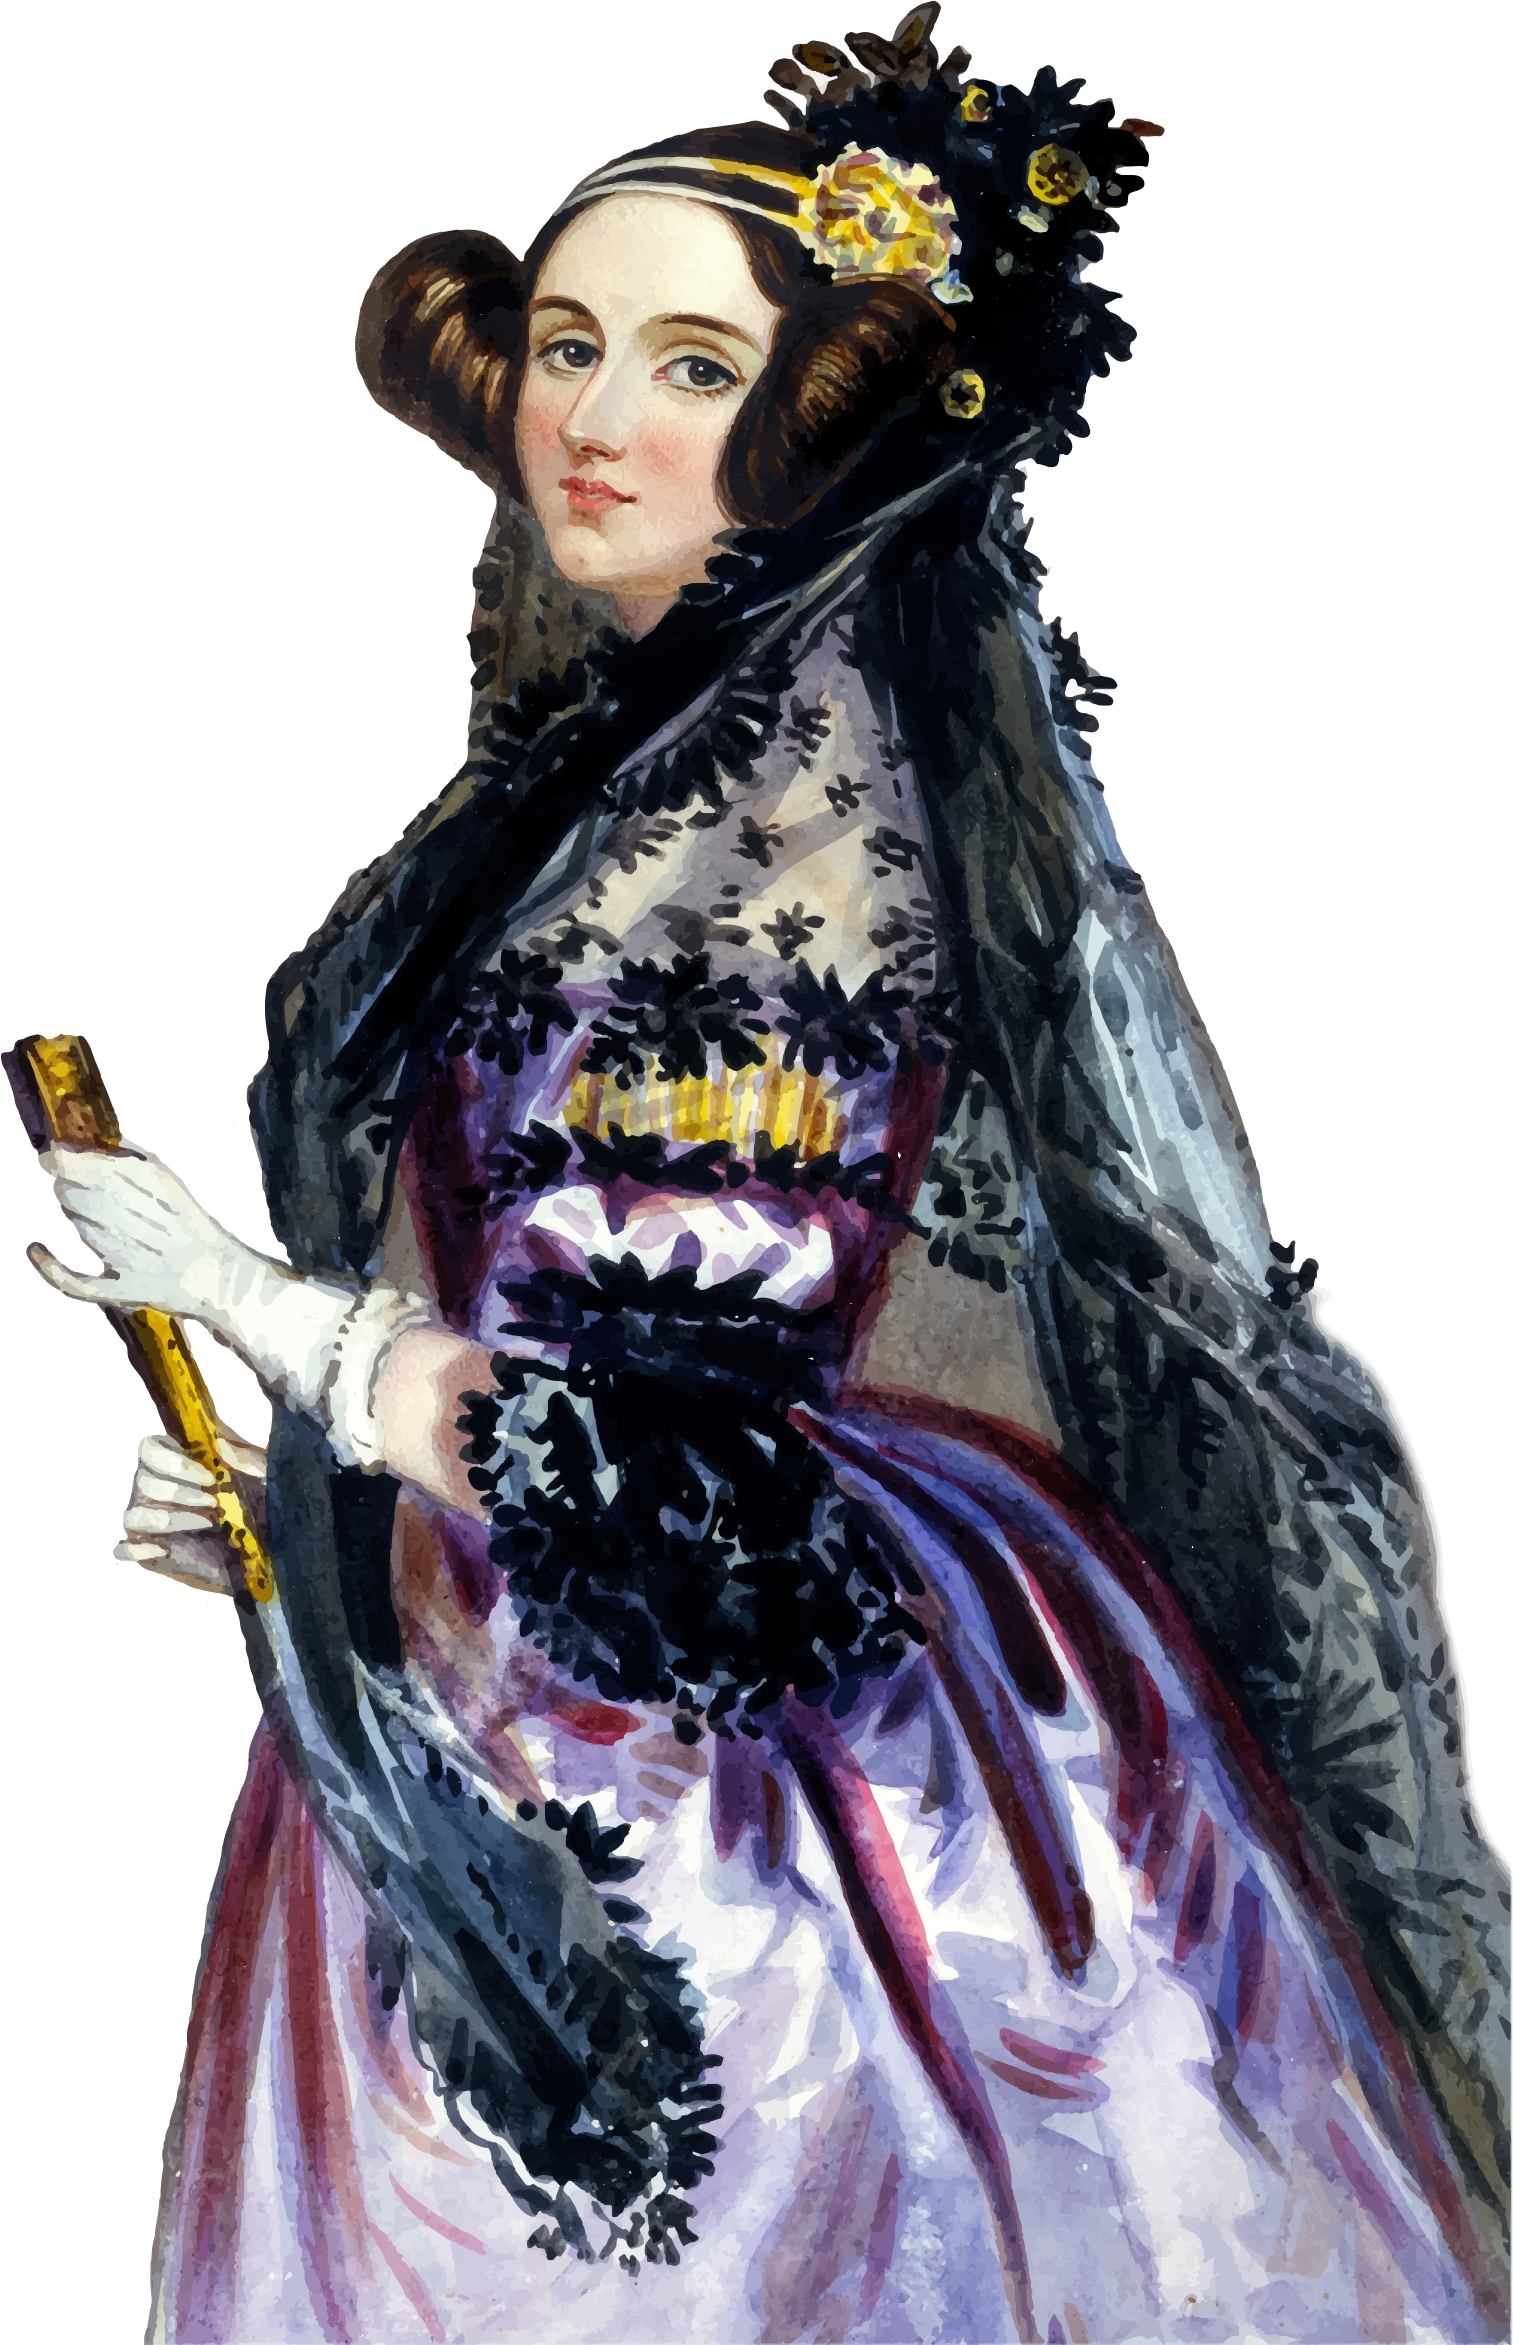
\includegraphics[scale=0.07]{lovelace}
	\caption{Ada Lovelace}
\end{figure}}

\only<2>{
	\begin{figure}
		\centering
		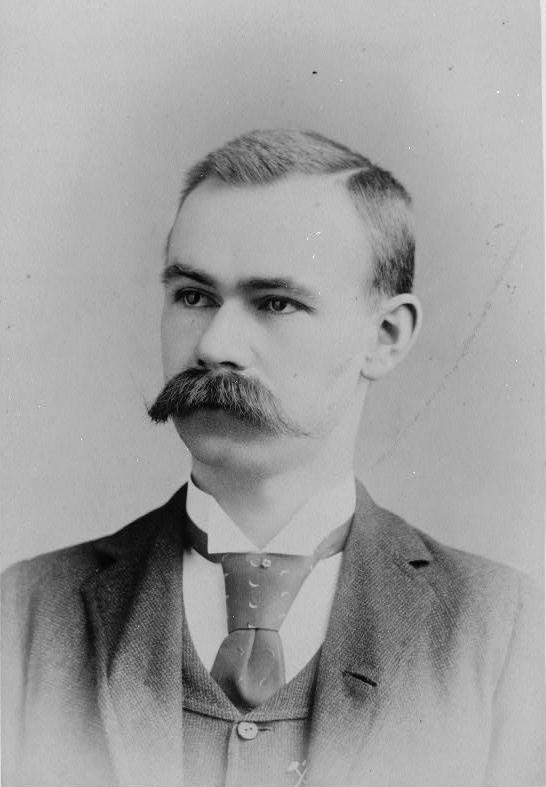
\includegraphics[scale=0.22]{hollerith}
		\caption{Herman Hollerith}
	\end{figure}}

\only<3>{
	\begin{figure}
		\centering
		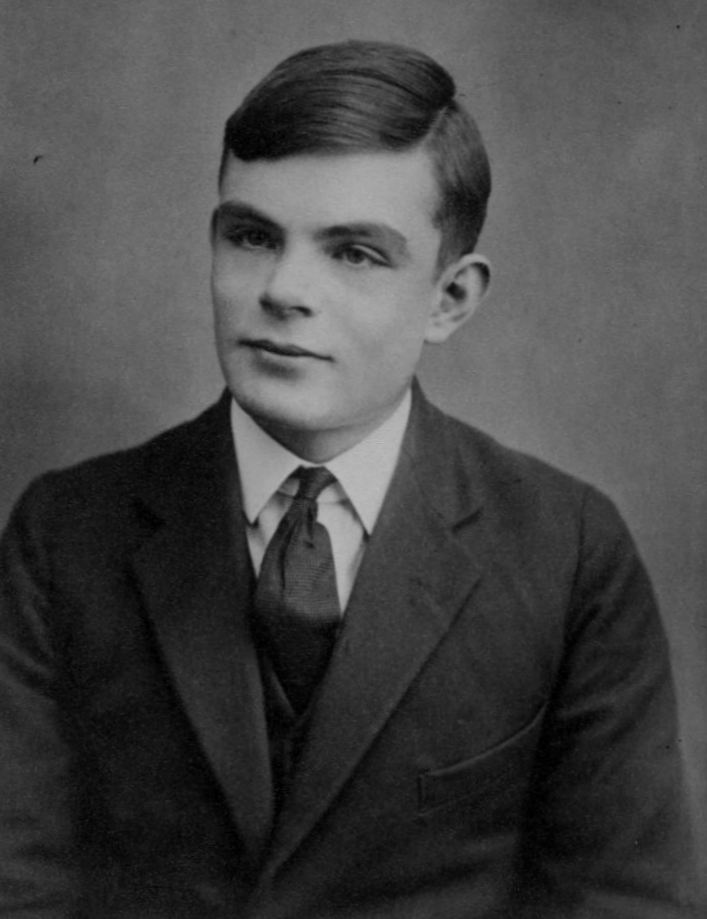
\includegraphics[scale=0.18]{turing}
		\caption{Alan Turing}
	\end{figure}}

\only<4>{
	\begin{figure}
		\centering
		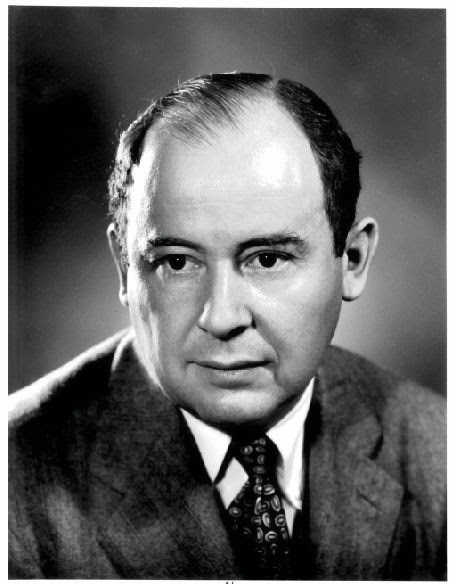
\includegraphics[scale=0.3]{neumann}
		\caption{John von Neumann}
	\end{figure}}

\only<5>{
	\begin{figure}
		\centering
		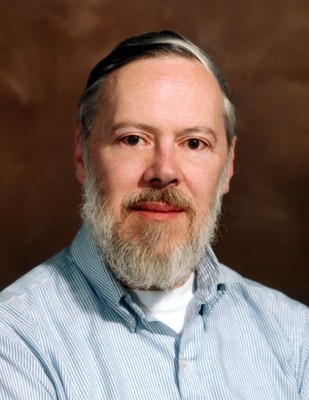
\includegraphics[scale=0.45]{ritchie}
		\caption{Dennis Ritchie}
	\end{figure}}
	
\only<6>{
	\begin{figure}
		\centering
		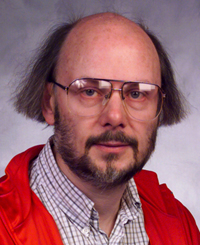
\includegraphics[scale=0.65]{stroustrup}
		\caption{Bjarne Stroustrup}
	\end{figure}}
	
\only<7>{
	\begin{figure}
		\centering
		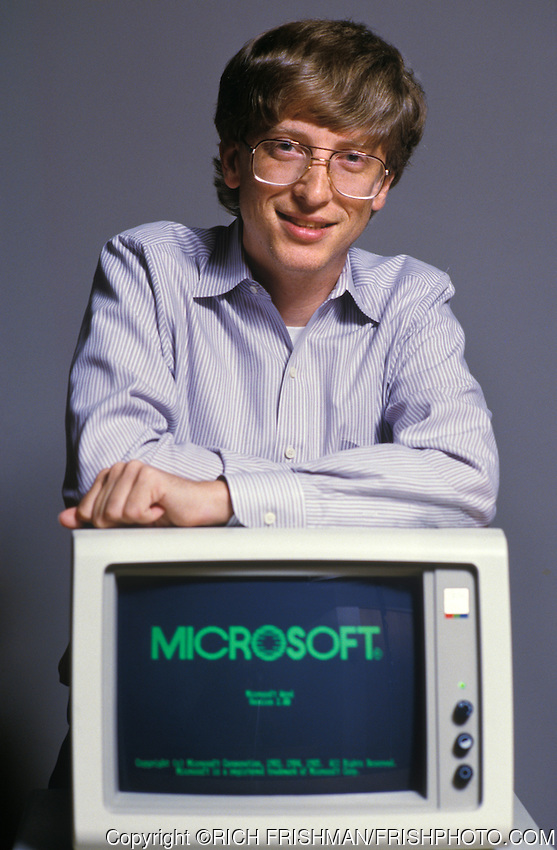
\includegraphics[scale=0.21]{gates}
		\caption{Bill Gates}
	\end{figure}}

\only<8>{
	\begin{figure}
		\centering
		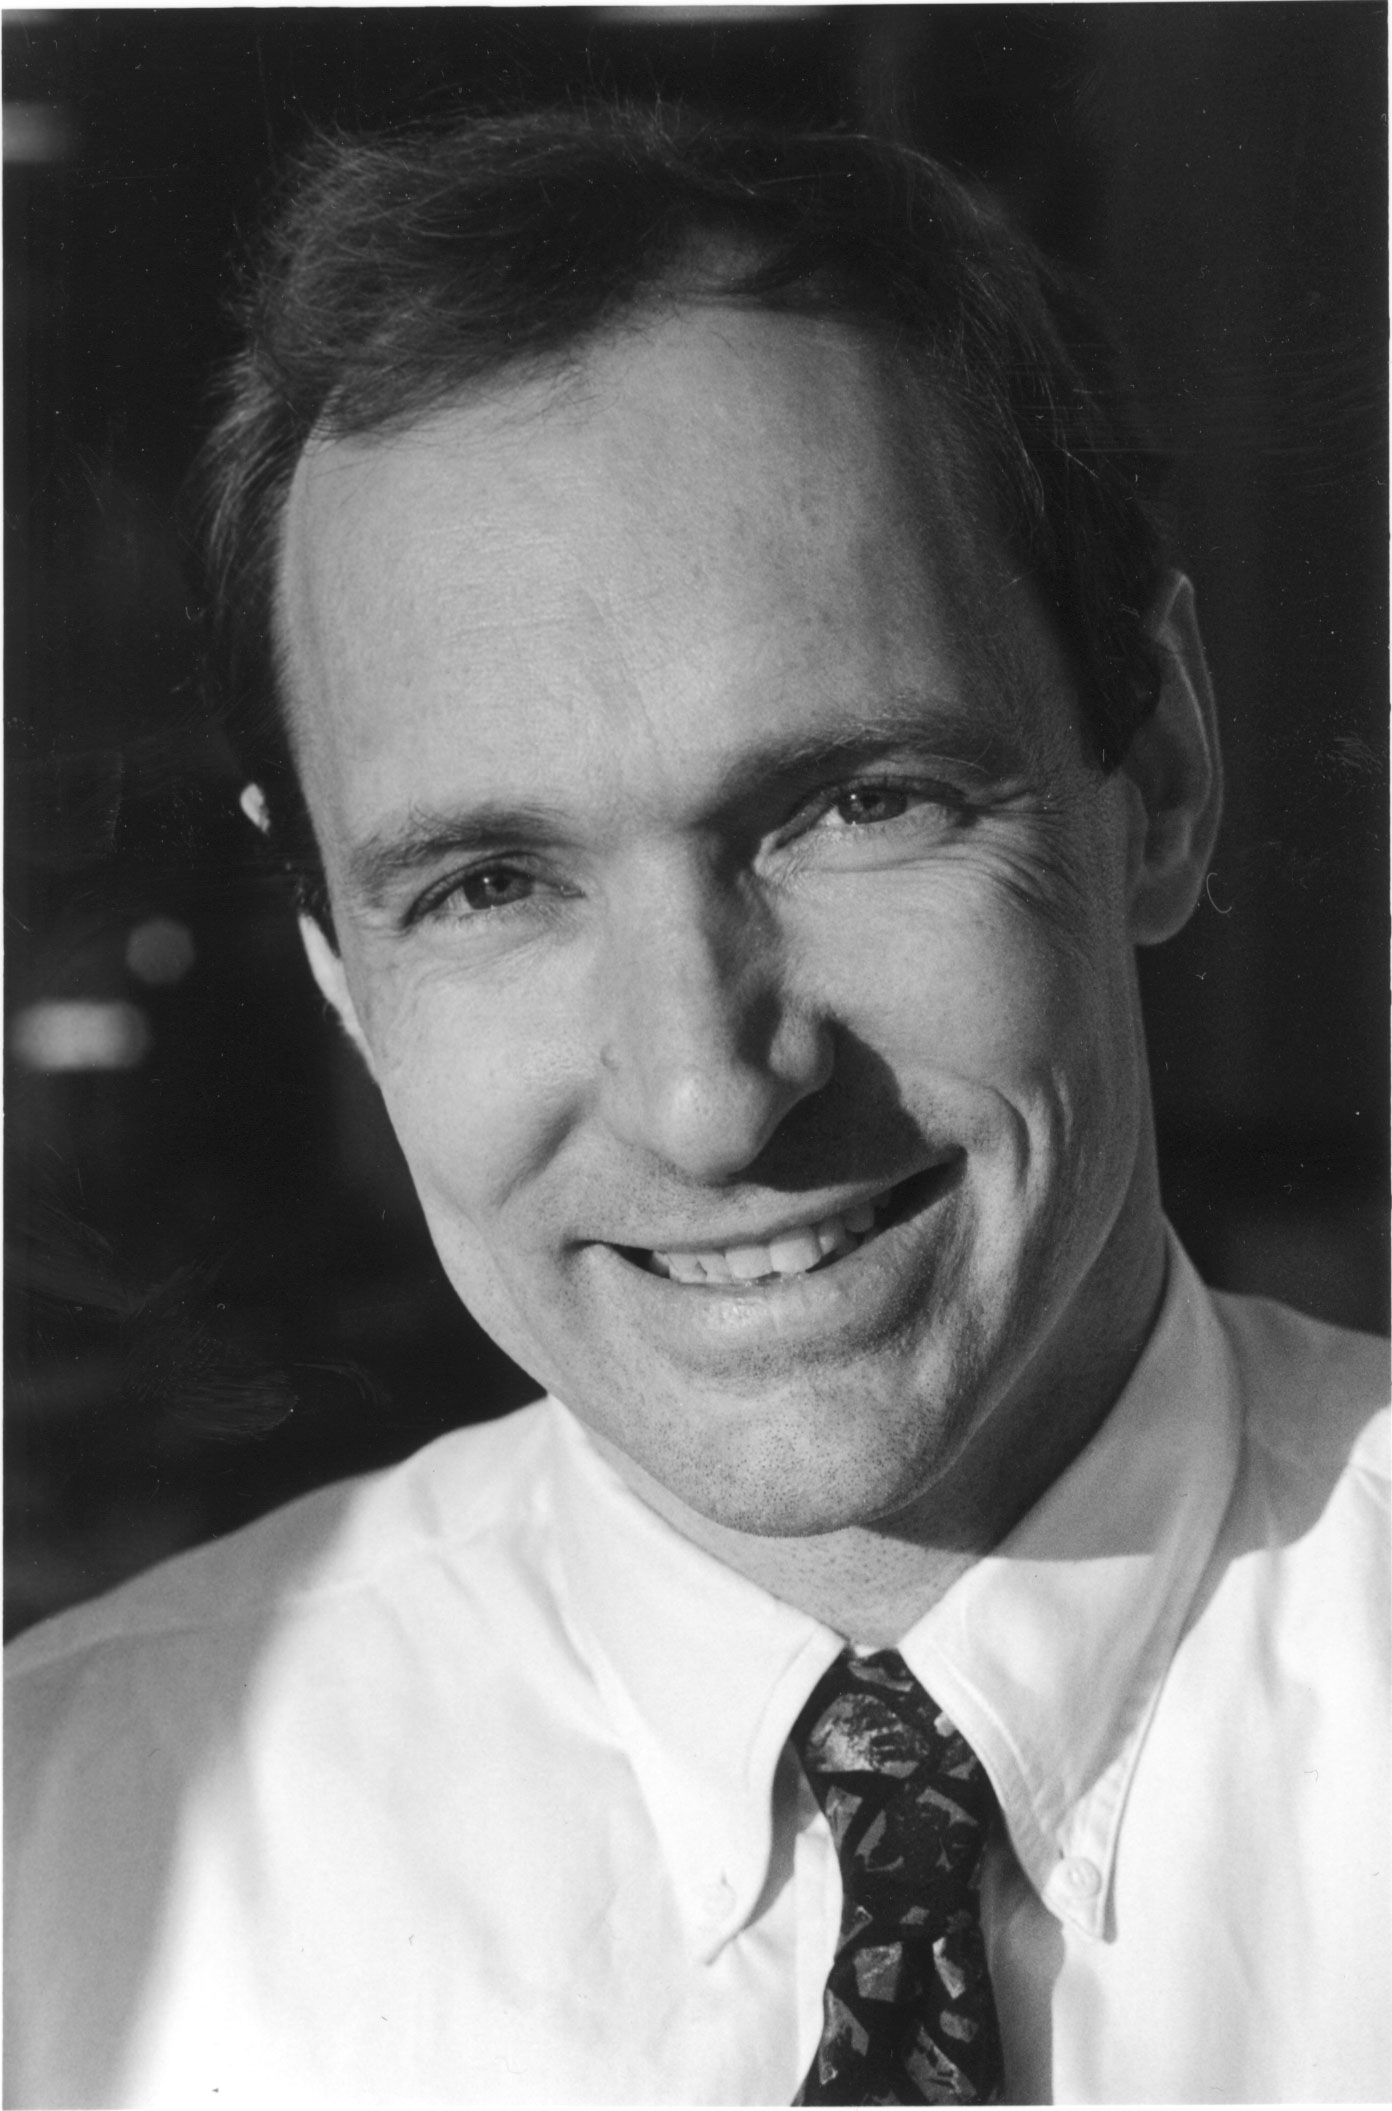
\includegraphics[scale=0.08]{bernerslee}
		\caption{Tim Berners-Lee}
	\end{figure}}

\only<9>{
	\begin{figure}
		\centering
		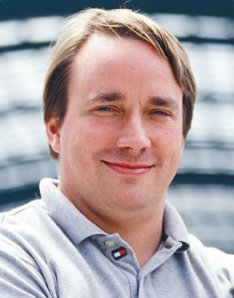
\includegraphics[scale=0.6]{torvalds}
		\caption{Linus Torvalds}
	\end{figure}}
	
\only<10>{
	\begin{figure}
		\centering
		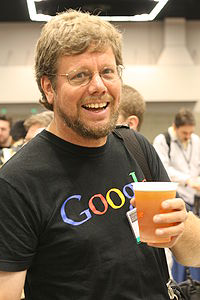
\includegraphics[scale=0.55]{vanrossum}
		\caption{Guido Van Rossum}
	\end{figure}}
\end{multicols}
\end{frame}

\section{Resolviendo problemas}

\begin{frame}[t]{Problema}\vspace{4pt}
\begin{figure}
	\centering
	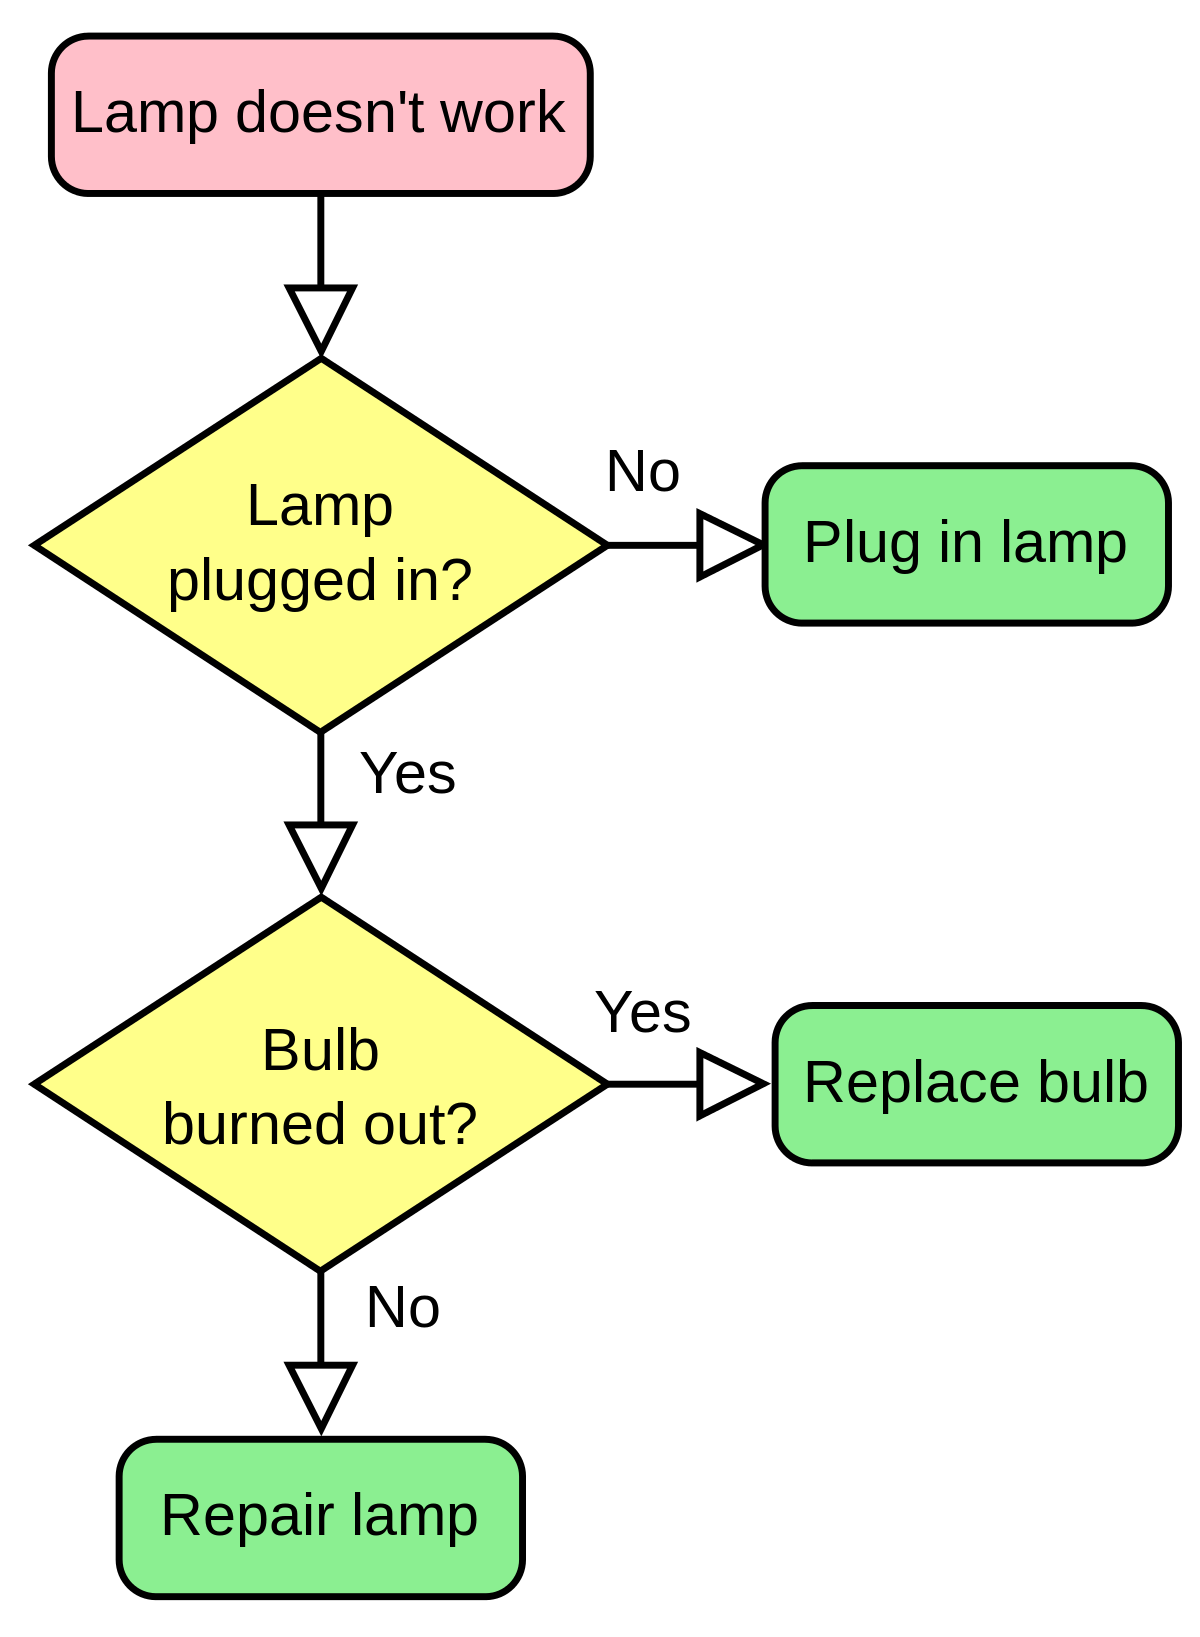
\includegraphics[scale=0.1]{problem}
	\caption{Diagrama de flujo}
\end{figure}	
\end{frame}

\begin{frame}[t]{Información contenida en el ADN}\vspace{4pt}
	\animategraphics[autoplay,loop,width=\linewidth, scale=0.9]{12}{dna-}{0}{29}	
\end{frame}


\begin{frame}[standout]
?`Preguntas?
\end{frame}

\begin{frame}[standout]
Tarea
\begin{itemize}
	\item Realizar cada una de las caras de un dado en diferentes archivos de Processing.
\end{itemize}
\end{frame}

\end{document}